This section describes the gimbal as a system, presenting the principles and how to mathematically model the dynamics.

\section{Reference Frames}
\label{secaorefframes}
To understand and accurately model a 2-DOF gimbal, it is essential to first divide the system into its primary components: the \textbf{inner gimbal}, the \textbf{outer gimbal}, and the \textbf{base}. The inner and outer gimbals provide movement in elevation ($\epsilon$) and azimuth ($\eta$), respectively, on their own reference frame. The base serves as the reference frame upon which the gimbals operate, and in this work, it is considered the inertial frame, meaning it is static and unaffected by external disturbances. It is assumed that all reference frames are orthogonal and their origin overlaps. Figure \ref{Gimbal2dg} ilustrates the reference frames in a 2-DOF gimbal, where $\mathbf{u^F_d}$ represents the unit vector of reference frame ``$F$'' in direction ``$d$''.

\begin{figure}[h]
 	\centering
 	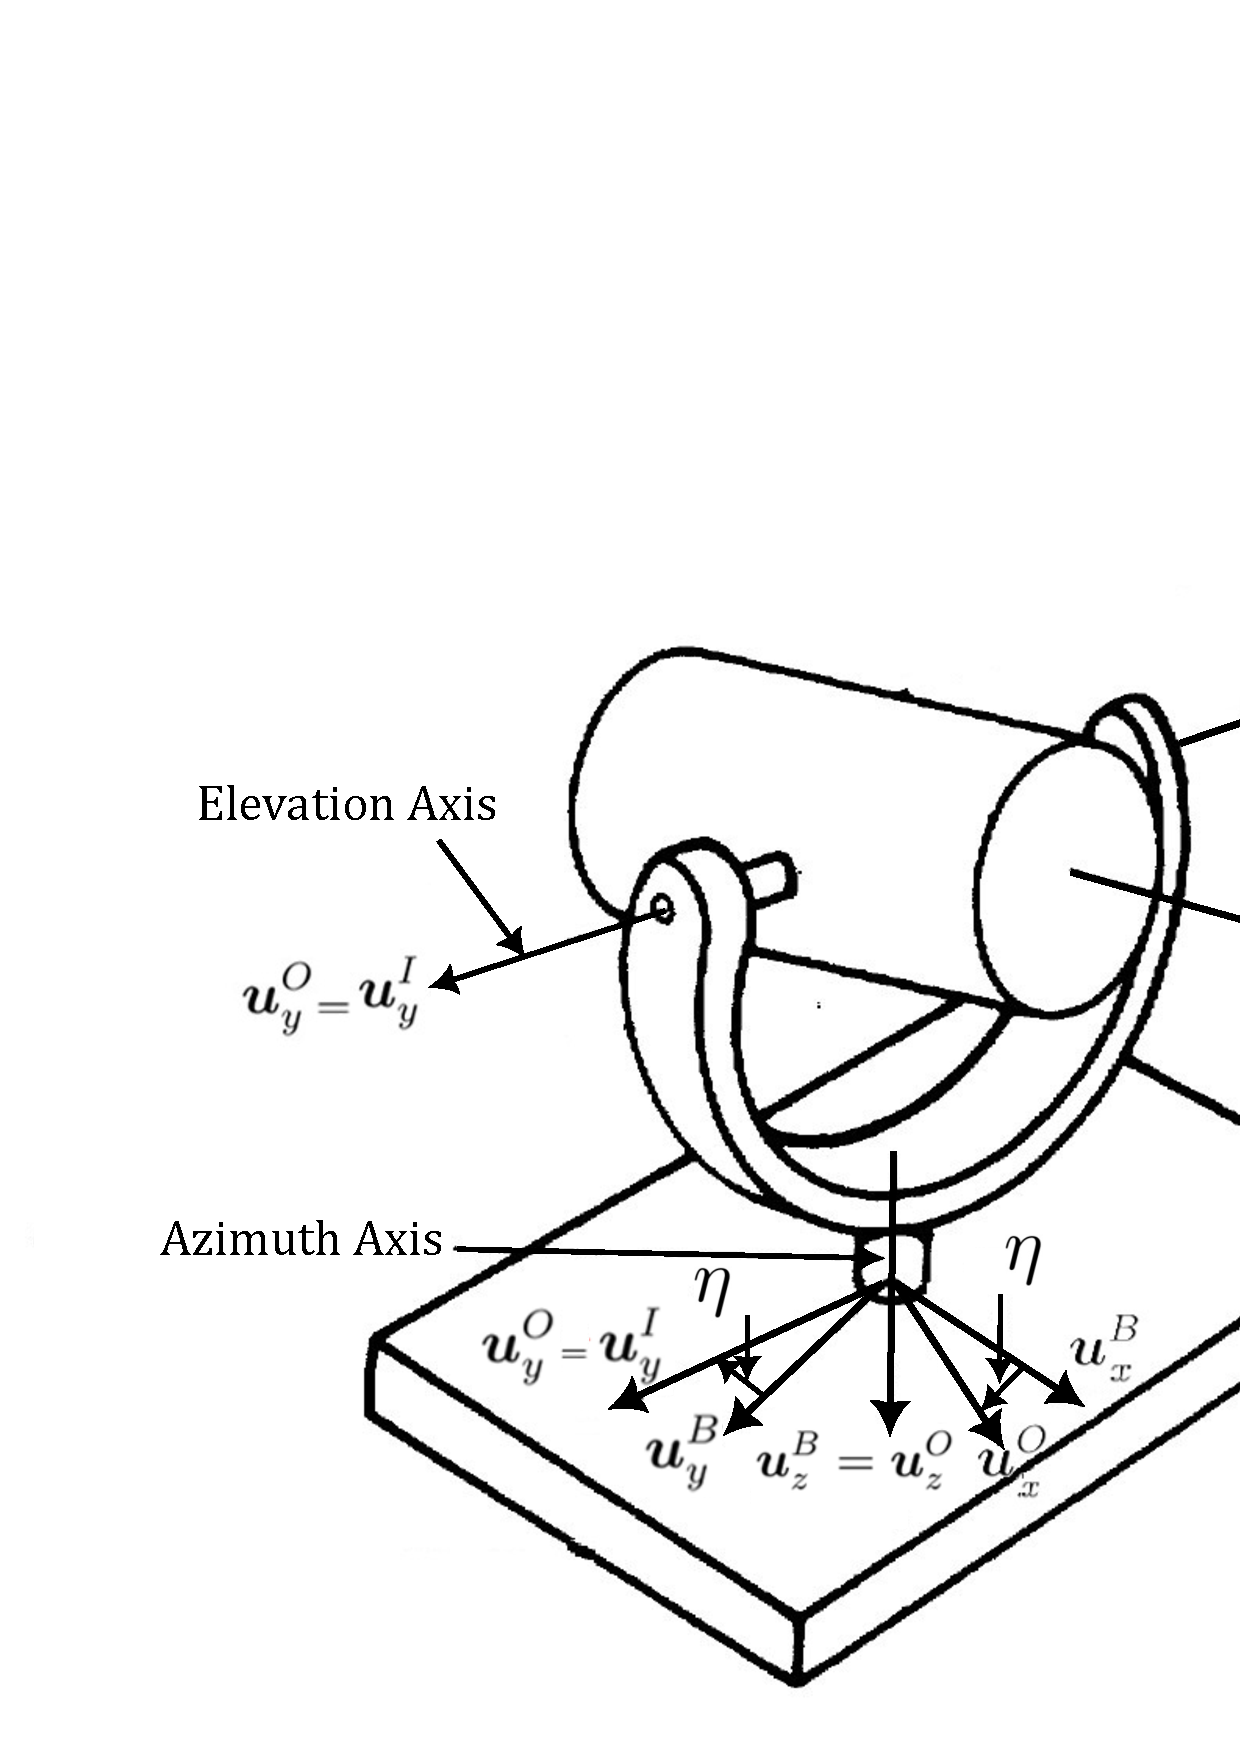
\includegraphics[scale = 0.4]{Cap6/Gimbal_final.jpg}
 	\caption{Reference frames of 2-DOF Gimbal.}\label{Gimbal2dg}
 \end{figure}

In which:
\begin{list}{}{}
\item \textbf{B}: Reference frame fixed to the gimbal base. In our case, coincident to intertal frame (earth).
 \item \textbf{O}: Reference frame fixed to the outer gimbal.
 \item \textbf{I}: Reference frame fixed to the Inner gimbal.
 \end{list}

And the unit vectors are expressed as:
\begin{align*}
     \mathbf{u_x} &= \begin{bmatrix}1\\0\\0\end{bmatrix} & \mathbf{u_y} &= \begin{bmatrix}0\\1\\0\end{bmatrix} & \mathbf{u_z} &= \begin{bmatrix}0\\0\\1\end{bmatrix}.
\end{align*}

 The relation between reference frames is estabilished by transformation matrices, which are thoroughly discussed in \cite{Done_1999}. For instance, a transformation matrix $\mathbf{T_{F_1 F_2}}$ projects a vector from reference frame $F_1$ to reference frame $F_2$. Taking into account that our system is not affected by disturbances in the \textbf{base} (B), the transformation matrices applied are:

 \begin{equation}
    \mathbb{T}_{BO}(\eta) = \mathbb{T}^T_{OB}(\eta) = \left[\begin{matrix} cos(\eta) & -sin(\eta) & 0 \\ sin(\eta) & cos(\eta) & 0 \\ 0 & 0 & 1 \end{matrix}\right]
 \end{equation}

  \begin{equation}
    \mathbb{T}_{OI}(\epsilon) = \mathbb{T}^T_{IO}(\epsilon) = \left[\begin{matrix} cos(\epsilon) & 0 & sin(\epsilon) \\ 0 & 1 & 0 \\ -sin(\epsilon) & 0 & cos(\epsilon) \end{matrix}\right]
 \end{equation}

 Given the orthogonal nature of reference frames, a fundamental characteristic of transformation matrices is observed: the multiplication of a transformation matrix by its transpose invariably produces the identity matrix ($\mathbf{I}$)

\begin{equation}
   \label{equacaoidentidade}
   \mathbb{T}^T\mathbb{T} = \mathbf{I}.
\end{equation}

 \section{Kinematics}
 The Kinematics of the gimbal refer to angular velocity and accelaration terms, which can be represented by X equations. To represent the inner and outer gimbal kinematics related to the inertial frame, the frames must be transformed to the reference frame of the gimbal base. A more detailed explanation is given in \citen{poyrazoglu_2017}.
 
 \subsection{Angular Velocity}
To express the velocity of each gimbal, firstly we stabilish the reference, which in our case will the the base (or inertial) frame. Hence, the velocity vector of inner and outer gimbals will be expressed as $\mathbf{\Omega}_{IB} = [\Omega_{IB_x},\Omega_{IB_y},\Omega_{IB_z}]^T$ and $\mathbf{\Omega}_{OB} = [\Omega_{OB_x},\Omega_{OB_y},\Omega_{OB_z}]^T$, respectively. Therefore, the velocity vectors can be written as

\begin{equation}
   \label{equacaoOB}
   \Omega_{OB_x} = 0
\end{equation}

\begin{equation}
   \Omega_{OB_y} = 0
\end{equation}

\begin{equation}
   \Omega_{OB_z} = \dot \eta
\end{equation}

for the outer gimbal, and

\begin{equation}
   \mathbf{\Omega}_{IB} = \dot \epsilon \mathbf{u}_y + \mathbb{T}_{IO}(\epsilon)  \mathbf{\Omega}_{OB} = \dot \epsilon \mathbf{u}_y + \mathbb{T}_{IO}(\epsilon)  \dot \eta \mathbf{u}_z,
\end{equation}

\begin{equation}
   \Omega_{IB_x} = -\dot \eta sin(\epsilon)
\end{equation}

\begin{equation}
   \Omega_{IB_y} = \dot \epsilon
\end{equation}

\begin{equation}
   \label{equacaoIB}
   \Omega_{IB_z} = \dot \eta cos(\epsilon)
\end{equation}

for the inner gimbal. Therefore, the resultant vectors can be expressed as

 \begin{equation}
    \mathbf{\Omega}_{OB} = \left[\begin{matrix} 0 \\ 0 \\ \dot \eta \end{matrix}\right]
 \end{equation}

 \begin{equation}
    \mathbf{\Omega}_{IB} = \left[\begin{matrix} -\dot \eta sin(\epsilon) \\ \dot \epsilon \\ \dot \eta cos(\epsilon) \end{matrix}\right].
 \end{equation}

 \subsection{Angular Acceleration}
The anglar acceleration is obtained by taking the first derivative of the velocity vector $\mathbf{\Omega}$ with respect to time. The angular acceleration of frame $F_1$ in relation to $F_2$ is expressed as $\bm{\alpha}_{F_1 F_2}$ = $[\alpha_{{F_1 F_2}_x}, \alpha_{{F_1 F_2}_y}, \alpha_{{F_1 F_2}_z}$]$^T$ .Therefore, the angular acceration vectors for our system are:

\begin{equation}
   \alpha_{OB_x} = 0
\end{equation}

\begin{equation}
   \alpha_{OB_y} = 0
\end{equation}

\begin{equation}
   \alpha_{OB_z} = \ddot \eta
\end{equation}

and

\begin{equation}
   \alpha_{IB_x} = - (\ddot \eta sin(\epsilon) + \dot \eta \dot \epsilon cos(\epsilon))
\end{equation}

\begin{equation}
   \alpha_{IB_y} = \ddot \epsilon 
\end{equation}

\begin{equation}
   \label{alphaelevacao}
   \alpha_{IB_z} = \ddot \eta cos(\epsilon) - \dot \eta \dot \epsilon sin(\epsilon)
\end{equation}

% To solve the term $\mathbb{\dot T}_{OI}(\epsilon)^T$ in equation \ref{alphaelevacao}, we will start by considering \citen{boiffier1998dynamics} explanation: ``The derivative with respect to the time \textit{t} of a vector $\mathbf{X}$ in the frame $\mathbf{F}_0$ ($\frac{d\mathbf{X^0}}{dt}$), is equal to the derivative of this vector $\mathbf{X}$ with respect to the time \textit{t} in the frame $\mathbf{F}_1$ ($\frac{d\mathbf{X^1}}{dt}$) to which must be added the cross product of \textbf{angular velocity} of the frame $\mathbf{F}_1$ relative to frame $\mathbf{F}_0$ ($\mathbf{\Omega}_{10}$), by the vector $\mathbf{X}$''. Therefore:

% \begin{equation}
%  \frac{d\mathbf{X^0}}{dt} = \frac{d\mathbf{X^1}}{dt} + \mathbf{\Omega}_{10} \times \mathbf{X}
% \end{equation}

% To apply this concept to transformation matrices, we must return to equation \ref{equacaoidentidade}. By derivating equation \ref{equacaoidentidade} with respect to time, the following relation is obtained:

% \begin{equation}
%    \mathbb{\dot T} ^T\mathbb{T} + \mathbb{T}^T \mathbb{\dot T} = 0
% \end{equation}

% Therefore, the equation can be written as

% \begin{equation}
%    \mathbb{\dot T} ^T\mathbb{T} = -\mathbb{T}^T \mathbb{\dot T}.
% \end{equation}

% According to \citen{boiffier1998dynamics}, $\mathbb{\dot T} ^T\mathbb{T}$ is a skew-symmetric matrix noted

% \begin{equation}
%    \mathbb{M}_{\Omega} = \left(\begin{matrix} 0 & -\Omega_z & \Omega_y \\ \Omega_z & 0 & -\Omega_x \\ -\Omega_y & \Omega_x & 0 \end{matrix}\right)
% \end{equation}

% where vector $\Omega$ is associated with matrix $\mathbb{M}_{\Omega}$, so that 

% \begin{equation}
%    \mathbb{M}_{\Omega} \mathbf{X} = \mathbf{\Omega} \times \mathbf{X}.
% \end{equation}

% Therefore, equation \ref{alphaelevacao} can be writen as

% \begin{equation*}
%    \bm{\alpha}_{IB_z} = \mathbb{M}_{\Omega_{IO}}\mathbb{T}_{IO}(\epsilon)  \dot \eta + \mathbb{T}_{IO}(\epsilon) \ddot \eta
% \end{equation*}

% \begin{equation}
%    \bm{\alpha}_{IB_z} = 
% \end{equation}

\section{Friction Model}
Friction between moving components represents a significant and often non-linear dynamic effect within mechanical systems, particularly prevalent in gimbal platforms. Friction is inherently present in the bearings supporting both the inner and outer gimbal axes, and its influence becomes particularly pronounced during changes in the direction of rotation.

For modeling purposes, the total friction force (or torque) can be broadly categorized into two primary types: viscous friction and Coulomb friction. The overall friction torque ($T_{\text{friction}}$) acting on the system is thus expressed as the sum of these two components:

\begin{equation*}
T_{\text{friction}} = T_{\text{viscous}} + T_{\text{coulomb}}
\end{equation*}

Where $T_{viscous}$ denotes the viscous friction torque and $T_{coulomb}$ represents the Coulomb friction torque. Viscous friction is characterized by its proportionality to the relative velocity between the moving surfaces, while Coulomb friction is non-linear in nature and is primarily based on the friction between two objects resulting from the applied normal force. In \citen{espinosa2016diseno}, these friction components are mathematically formulated as:
    \begin{equation}
      \label{atritoviscoso}
    T_{\text{viscous}} = k_{\text{vf}} \Omega
    \end{equation}
    In \ref{atritoviscoso}, $k_{\text{vf}}$ is the viscous friction coefficient between the moving parts in the gimbal system, and $\dot{\epsilon}$ represents the angular velocity of the inner gimbal.

    \begin{equation}
      \label{atritocoulomb}
    T_{\text{coulomb}} = k_{\text{cf}} \text{sign}(\Omega)
    \end{equation}
    In equation \ref{atritocoulomb}, $k_{\text{cf}}$ is the Coulomb friction coefficient, and $\text{sign}(\dot{\epsilon})$ is the sign function of the angular velocity, ensuring that the friction torque opposes the direction of motion.

This detailed modeling of friction results in a more realistic dynamic behavior of the gimbal system, allowing for a more accurate simulation and subsequent controller design that accounts for these inherent non-linearities.

\section{Gimbal Dynamics}
To obtain the equations describing the gimbal's dynamics, we will employ the Newton-Euler mechanics. This approach, based on applying Newton's laws for translation and Euler's laws for rotation to each rigid body in the system, is widely used in the modeling of mechatronic and robotic systems, as detailed in works such as \citen{boiffier1998dynamics}.

The choice of the Newton-Euler method is justified by its ability to provide a direct representation of the relationships between applied forces/torques and the resulting motion, making it particularly useful for systems with rotational joints like gimbals. To simplify the derivation of the equations and focus on the central aspects of tracking control, premises are adopted regarding mass distribution and rotation axes, such as \textbf{homogeneous mass distribution}, which is the assumption that mass is homogeneously distributed within the gimbals and the \textbf{alignment with principal axes of inertia}, ensuring that the axes of rotation coincide exactly with the principal axes of inertia of each link. These simplifications implies that products of inertia are null, resulting in diagonal inertia tensors. Such an approach is common in initial models to reduce complexity and is explored in works such as \citen{poyrazoglu_2017} and \citen{espinosa2016diseno}, which also use this premise to simplify the modeling of gimbal dynamics. Another assumption is the \textbf{fixed base}, in which the base is considered fixed and represents the system's inertial reference frame. This means that no movements or external disturbances act upon the base, simplifying the kinematic and dynamic equations by eliminating terms related to the supporting platform's dynamics.

These premises allow for a clearer derivation of the fundamental equations, which will serve as the basis for the subsequent incorporation of specific nonlinearities of the system and the actuator, in line with the objective of this work.

\subsection{Inner Gimbal}
The angular momentum of the inner gimbal about the pivot point P relative to the inner gimbal frame is
\begin{equation}
   \mathbf{H}^I_{I,P} = \mathbb{I}^I_P \mathbf{\Omega}_{IB}
\end{equation}
Here, $\mathbb{I}^I_P$ represents the inertia tensor of the decoupled inner gimbal, calculated about the pivot point, and $\mathbf{\Omega}_{IB}$ denotes the inner gimbal's angular velocity vector relative to the Earth frame. The total moment exerted on the inner gimbal is obtained from the first-order time derivative of its angular momentum. Building upon calculations presented in \citen{boiffier1998dynamics}, Euler's equation for the inner gimbal, specifically about its pivot point, is thus formulated as:
\begin{equation}
   \label{momento total}
   \mathbf{M}_{OI} = \frac{d\mathbf{H}^O_{I,P}}{dt} = \mathbb{I}^I_P \bm{\alpha}_{IB} + \mathbf{\Omega}_{IB} \times \mathbf{H}^I_{IP}.
\end{equation}
In equation \ref{momento total}, $\mathbf{H}^O_{I,P}$ is the angular momentum of the inner gimbal about the pivot point P relative to the outer gimbal frame, and $\bm{\alpha}_{IB}$ is the inner gimbal's angular acceleration vector. Using the premises stated in the beginning of this section, the inertia tensor and, therefore, the vector representing the total moment exerted on the inner gimbal can be expressed as
\begin{equation}
   \mathbb{I}^I_P = \left[ \begin{matrix}I^I_x & 0 & 0 \\ 0 & I^I_y & 0 \\ 0 & 0 & I^I_z\end{matrix}\right]
\end{equation}
\begin{equation}
   \mathbf{M}_{OI} = \left[ \begin{matrix}I^I_x \alpha_{IB_x} + (I^I_z - I^I_y) \Omega_{IB_y} \Omega_{IB_z} \\ I^I_y \alpha_{IB_y} + (I^I_x - I^I_z) \Omega_{IB_x} \Omega_{IB_z} \\ I^I_z \alpha_{IB_z} + (I^I_y - I^I_x) \Omega_{IB_x} \Omega_{IB_y}\end{matrix}\right]
\end{equation}
Including the effects of friction torque in the total moment, and consiering that torque is transfered from outer gimbal to inner gimbal along y axis, therefore neglecting the components in x and z axes, the resultant vector is now
\begin{equation}
   \left[\begin{matrix} 0 \\ T_{m_I} + T_{\text{Friction}_{OI}} \\ 0\end{matrix}\right] = \left[ \begin{matrix} 0 \\ I^I_y \alpha_{IB_y} + (I^I_x - I^I_z) \Omega_{IB_x} \Omega_{IB_z} \\ 0 \end{matrix}\right],
\end{equation}
which gives us the equation for elevation torque for the angular momentum in the y axis for the inner gimbal:
\begin{equation}
   \label{Momento angular y inner}
   T_{m_I} + T_{\text{Friction}_{OI}} = I^I_y \alpha_{IB_y} + (I^I_x - I^I_z) \Omega_{IB_x} \Omega_{IB_z} 
\end{equation}
In equation \ref{Momento angular y inner}, $T_{m_I}$ is the torque transmited from the outer gimbal to the inner gimbal by an electrical motor, and $T_{\text{Friction}_{OI}}$ is the friction torque between outer and inner gimbals.

\subsection{Outer Gimbal}
The angular momentum of the outer gimbal about the pivot point P relative to the outer gimbal frame is

\begin{equation}
   \mathbf{H}^O_{O,P} = \mathbb{I}^O_P \mathbf{\Omega}_{OB} + \mathbb{T}_{IO} \mathbf{H}^I_{I,P}
\end{equation}

Here, $\mathbb{I}^O_P$ represents the inertia tensor of the decoupled inner gimbal, calculated about the pivot point, and $\mathbf{\Omega}_{OB}$ denotes the inner gimbal's angular velocity vector relative to the Earth frame. It is important to notice that this equation already consider the influence of the inner gimbal in the outer gimbal's angular moment. Applying the same considerations used in equation \ref{momento total}, Euler's equation of the outer gimbal about the pivot point is expressed as
\begin{equation}
\mathbf{M}_{BO} + \mathbf{M}_{IO} = \frac{d\bm{H}^B_{O,P}}{dt}
\end{equation}

\begin{equation}
   \label{momento total outer gimbal}
   \frac{d\bm{H}^B_{O,P}}{dt} = \mathbb{I}^O_P \bm{\alpha}_{OB} + \mathbb{\dot T}_{IO} \mathbb{I}^I_P \bm{\Omega}_{IB} + \mathbb{T}_{IO} \mathbb{I}^I_P \bm{\alpha}_{IB} + \bm{\Omega}_{OB} \times (\mathbb{I}^O_P \bm{\Omega}_{OB} + \mathbb{T}_{IO} \mathbb{I}^I_P \bm{\Omega}_{IB})
\end{equation}

Where $\mathbf{H}^B_{O,P}$ is the angular momentum of the outer gimbal about the pivot point P relative to the base frame. By expanding the terms in equation \ref{momento total outer gimbal}, and under the assumption that torque is transfered from base to outer gimbal along z axis, thus $M_{IO_x}$ = $M_{IO_y}$ = $M_{BO_x}$ = $M_{BO_y}$ = 0, the resultant vectors for $M_{BO}$ and $M_{IO}$ are:

\begin{align*}
     \mathbf{M}_{IO} &= \left[\begin{matrix}0 \\ 0 \\ T_{\text{Friction}_{IO}}\end{matrix}\right] & \mathbf{M}_{BO} &= \left[\begin{matrix}0 \\ 0 \\ T_{m_O} + T_{\text{Friction}_{BO}}\end{matrix}\right].
\end{align*}

In this case, $T_{\text{Friction}_{BO}}$ and $T_{\text{Friction}_{IO}}$ indicate the friction torques between the base and the outer gimbal, and between the inner and outer gimbals, respectively, with $T_{m_O}$ being the motor torque applied to the outer gimbal. Due to the alignment of the rotation axes of the base and the outer gimbal along the z axis, the sum of $T_{m_O}$ and $T_{\text{Friction}_{BO}}$ is directly transmitted to the outer gimbal, whereas $T_{\text{Friction}_{IO}}$ is a friction torque transferred indirectly. Therefore, the equation of motion for the outer gimbal on the z axis is given by
\begin{equation*}
   T_{m_O} + T_{\text{Friction}_{BO}} + T_{\text{Friction}_{IO}} = 
\end{equation*}

\begin{equation}
I^O_z \alpha_{{OB}_z} + I^I_z \alpha_{{IB}_z} cos(\epsilon) + I^I_x \alpha_{{IB}_x} sin(\epsilon) - I^I_x \Omega_{{IB}_x} \Omega_{{IB}_y}  cos(\epsilon) + I^I_z\Omega_{{IB}_z} \Omega_{{IB}_y} sin(\epsilon)
\end{equation}